\chapter{Foundations}
\label{ch:fundamentals}

% We need the fundamentals to understand the background underlying the problem and the solution space.

In this section, we explain the foundational concepts of this master thesis. We begin with the explanation of \gls{kgqa} and \glspl{kg}. Then, we provide an overview of \glspl{llm} and describe how \gls{grag} can unify the abilities of \glspl{llm} with the structured knowledge from \glspl{kg} for answering natural language questions. Following this, we provide an explanation of \gls{ann}, a fundamental concept of our HubLink approach. Next, we describe the metrics that are commonly used in \gls{rag} research, which we will also be using in our evaluation. Lastly, we define the term taxonomy within the scope of the thesis and explain its construction and evaluation concepts.




\section{Knowledge Graphs}
\label{sec:fundamentals_knowledge_graphs}

\acrfullpl{kg} represent information as structured networks. In these networks, nodes typically denote entities such as individuals, locations, publications, or abstract concepts, while the edges signify the relationships that connect these entities \cite{banerjee_knowledge_2024,pan_unifying_2024}. Although there are numerous definitions for \glspl{kg}, many prominent implementations are modeled using the \gls{rdf} \cite{ehrlinger_towards_2016}. \gls{rdf} provides a graph-based data model standardized by the World Wide Web Consortium (W3C) \cite{wood_rdf_2014}. Consequently, for the scope of this thesis, the term \gls{kg} will specifically refer to an \gls{rdf} graph.

The fundamental unit of an \gls{rdf} graph is the \emph{triple}, a tuple comprising three components: a subject, a predicate, and an object \cite{pan_unifying_2024,wood_rdf_2014,ji_survey_2022}. Following the W3C standard, an \gls{rdf} graph G is formally defined as a set of such triples:
\[
G = \{\, t = (s, p, o) \mid s \in \mathcal{I} \cup \mathcal{B},\; p \in \mathcal{I},\; o \in \mathcal{I} \cup \mathcal{B} \cup \mathcal{L} \,\},
\]
where:
\begin{itemize}
  \item \(\mathcal{I}\) is the set of \glspl{iri}, which uniquely identify resources,
  \item \(\mathcal{B}\) is the set of blank nodes representing resources without a global identifier,
  \item \(\mathcal{L}\) is the set of literals, which are atomic pieces of information (e.g., strings, numbers).
\end{itemize}

Furthermore, a triple \(t = (s, p, o)\) consists of:
\begin{itemize}
  \item \emph{Subject} \(s\): The resource being described, which is either an \gls{iri} or a blank node.
  \item \emph{Predicate} \(p\): A property (or relation) represented as an \gls{iri} that links the subject to the object.
  \item \emph{Object} \(o\): The target or value of the relationship, which may be an \gls{iri}, a blank node, or a literal.
\end{itemize}

The key characteristics of a \gls{kg} have been expressed by \autocite{verma_scholarly_2023}: 
\begin{itemize}
    \item The structure of a \gls{kg} depends on the use of an ontology, which defines the concepts, properties, and associations across a single or multiple domains.
    \item A \gls{kg} is formulated in a triple format and is often stored as an \gls{rdf} graph.
    \item To create the \gls{kg}, knowledge is curated from structured and unstructured sources.
    \item The \gls{kg} is stored in a graph database management system and queried using adaptive querying languages such as CYPHER, SPARQL, SQL, and API calls to retrieve data from the graph.
\end{itemize}

\subsection{Research Knowledge Graphs}

\glspl{kg} are classified based on the information they store. Several categories are recognized in the literature \cite{pan_unifying_2024}: \emph{Encyclopedic \glspl{kg}} aim to represent real-world knowledge, often integrating information from diverse sources like encyclopedias, expert input, and databases. \emph{Commonsense \glspl{kg}} focus on modeling tacit, everyday knowledge and the relationships between common concepts. \emph{Domain-specific \glspl{kg}} contain specialized information pertinent to particular fields. Furthermore, \emph{Multi-modal \glspl{kg}} extend the traditional graph structure to incorporate information from various modalities, including images, audio, and video.

Another type of \glspl{kg} are \acrfullpl{rkg}, which are graphs focused on scholarly communication. Although an \gls{rkg} can also store typical data such as people, documents, datasets, and institutions, it also includes relationships between problems, methods, and results. A distinguishing feature is the representation of statements extracted from scientific articles as semantic resources within the graph. These resources are explicitly linked to their source articles, enabling direct traceability of information provenance. \cite{auer_towards_2018}

\textcite{karras_divide_2023} propose a categorization of \glspl{rkg} into \emph{generic} and \emph{specific} types. Generic \glspl{rkg} primarily utilize bibliographic metadata to structure entities and relationships. Prominent examples include the \emph{Microsoft Academic Knowledge Graph} \cite{ghidini_microsoft_2019,farber_microsoft_2022}, \emph{OpenAlex} \cite{priem_openalex_2022}, \emph{Springer Nature SciGraph} \cite{hammond_data_2017}, \emph{Semantic Scholar Literature Graph} \cite{kinney_semantic_2023}, \emph{OpenAIRE Research Graph} \cite{manghi_data_2012}, \emph{Research Graph} \cite{aryani_research_2017}, and the \emph{Scholarly Link Exchange (Scholix)} framework \cite{burton_scholix_2017}. In contrast, specific \glspl{rkg} focus on storing detailed scientific data in addition to bibliographic metadata. These graphs are employed to describe and link research artifacts and entities, often tailored to particular scientific topics or domains. Notable examples are \emph{CovidGraph} \cite{domingo-fernandez_covid-19_2021}, \emph{SoftwareKG} \cite{harth_investigating_2020}, the \emph{Computer Science Knowledge Graph (CS-KG)} \cite{sattler_cs-kg_2022}, the \emph{Cooperation Databank (CoDa)} \cite{spadaro_cooperation_2022}, and \emph{OpenBiodiv} \cite{penev_openbiodiv_2019}.


\subsection{The Open Research Knowledge Graph (ORKG)}

Beyond the generic and specific classifications, the \acrfull{orkg} presents a distinct approach by aiming to organize topic-specific scientific data semantically across diverse research domains \cite{karras_divide_2023}.

The \gls{orkg} is an \gls{rkg} that stores scientific articles along with their contributions as semantic units. It provides the infrastructure for acquiring, curating, publishing, and processing semantic scientific knowledge with the goal of making scientific findings more accessible to both humans and machines \cite{jaradeh_open_2019-1}. The graph is publicly accessible through a website\footnote{\url{https://orkg.org/} [last accessed on 21.12.2024]} and is maintained by the \gls{orkg} community. New entries can be added by any user, with entry quality being monitored by administrators. At the time of writing this thesis, the graph contains over 33,800 articles across more than 700 different research fields\footnote{\url{https://orkg.org/stats} [last accessed on 21.12.2024]}.

\paragraph{Data Model} Knowledge in the \gls{orkg} is stored closely following the \gls{rdf} format, meaning that at the core, the graph is stored in triples, which are also referred to as \emph{statements}. As detailed in \autoref{tab:orkg_statements}, each component of a statement accommodates specific types of information. Subjects and objects can represent resources, properties, or classes, whereas predicates are restricted to properties. Literals are used for atomic data, such as text, numbers, or dates, and are used exclusively as objects within statements. Furthermore, the \gls{orkg} system automatically assigns a unique identifier (ID) to each resource, property, class, and literal instance. \cite[21-22]{ilangovan_open_2024}

\begin{table}[t]
\centering
\begin{tabular}{|l|l|l|}
\hline
\textbf{Subject} & \textbf{Predicate} & \textbf{Object} \\ \hline
\{ Resource, Property, Class \} & Property & \{ Resource, Property, Class, Literal \} \\ \hline
\end{tabular}
\caption[Permitted ORKG Statement Types]{The permitted types in ORKG statements for the Subject, Predicate, and Object in a triple, based on \cite[21]{ilangovan_open_2024}.}
\label{tab:orkg_statements}
\end{table}

\paragraph{Content Types} Information stored in the \gls{orkg} is organized using distinct content types. A primary content type is the \emph{paper}. When a paper is added, the system automatically populates associated metadata, including its DOI, title, research field, authors, publication date, venue, and URL. Another crucial content type is the \emph{contribution}, which allows users to add structured data describing the research findings presented in the paper, extending beyond simple metadata. These contributions can subsequently be utilized within \emph{comparisons}, another \gls{orkg} content type. Comparisons facilitate the contrasting of research findings across multiple papers and can be semi-automatically generated by the system to identify shared properties among different contributions. \cite[22]{ilangovan_open_2024}

\paragraph{Contribution Templates} To promote standardization in the way contributions are structured, the \gls{orkg} offers \emph{templates}. These templates implement a subset of the Shapes Constraint Language (SHACL) \cite{knublauch_shapes_2017} and define the expected structure for contributions related to specific types of research descriptions. Intended for creation by domain experts, templates specify constraints and requirements, ensuring consistency and quality in the data entered for contributions within particular research areas. \cite[58-60]{ilangovan_open_2024}

\paragraph{Research Fields} The concept of \emph{research fields} serves as a primary organizational mechanism within the \gls{orkg}. Research fields can be associated with various content types (papers, contributions, comparisons, templates, etc.) to enable the grouping and categorization of related content within the graph. \cite[29-30]{ilangovan_open_2024}

\paragraph{Lists} \emph{Lists} provide another organizational tool in the \gls{orkg}. They allow users to group related papers thematically or for specific purposes without necessarily requiring the addition of detailed structured data for each paper within the list. \cite[28-29]{ilangovan_open_2024}

\begin{figure}
    \centering
    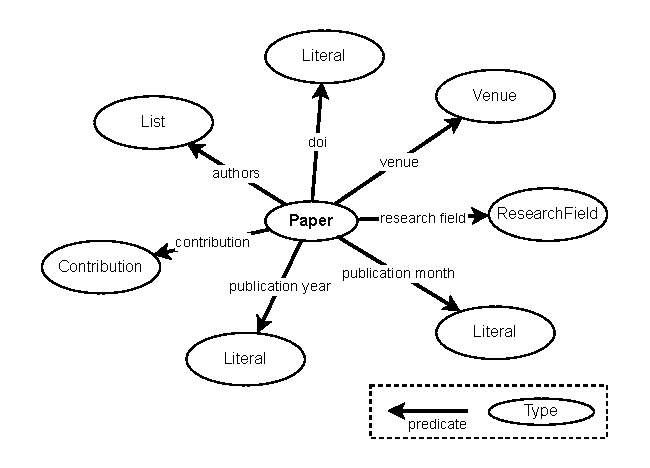
\includegraphics[width=0.7\linewidth]{figures/orkg/figures-orkg_structure.drawio.pdf}
    \caption[Schematic Representation of ORKG Publication Data]{Schematic representation of how publication data is structured in the ORKG, illustrating the root entity \emph{Paper} and its linkage to metadata and \emph{Contribution} entities.}
    \label{fig:orkg_structure}
\end{figure}

\paragraph{Storing Publications} As previously mentioned, scientific publications are represented in the \gls{orkg} using the \emph{paper} content type. Interaction with these paper entities forms the principal mode of engagement with the \gls{orkg} relevant to this thesis. \autoref{fig:orkg_structure} depicts the organizational structure for storing publication data. The diagram illustrates that the paper entity serves as the central node for publication information. All associated data, including metadata and one or more contributions detailing the research content, are linked to this paper entity using statements.

\subsection{The KARAGEN Approach for Question Answering on the ORKG}

\gls{karagen} is an approach for implementing a \gls{qa} system on the \gls{orkg} graph. The goal is to take advantage of the complementary strengths of \glspl{llm} and \gls{kg}. In this relationship, the \gls{kg} provides a structured data foundation in which information is stored in an interconnected network of entities and their relationships. The benefit of the graph is the ability to semantically link information, thus preserving the context and relationships between pieces of knowledge. On the other hand, \glspl{llm} excel in interpreting and generating natural language, with their advantage being that users can formulate their queries in natural language instead of relying on keyword-based queries. \cite{kaplan_combining_2024}

\begin{figure}[t]
    \centering
    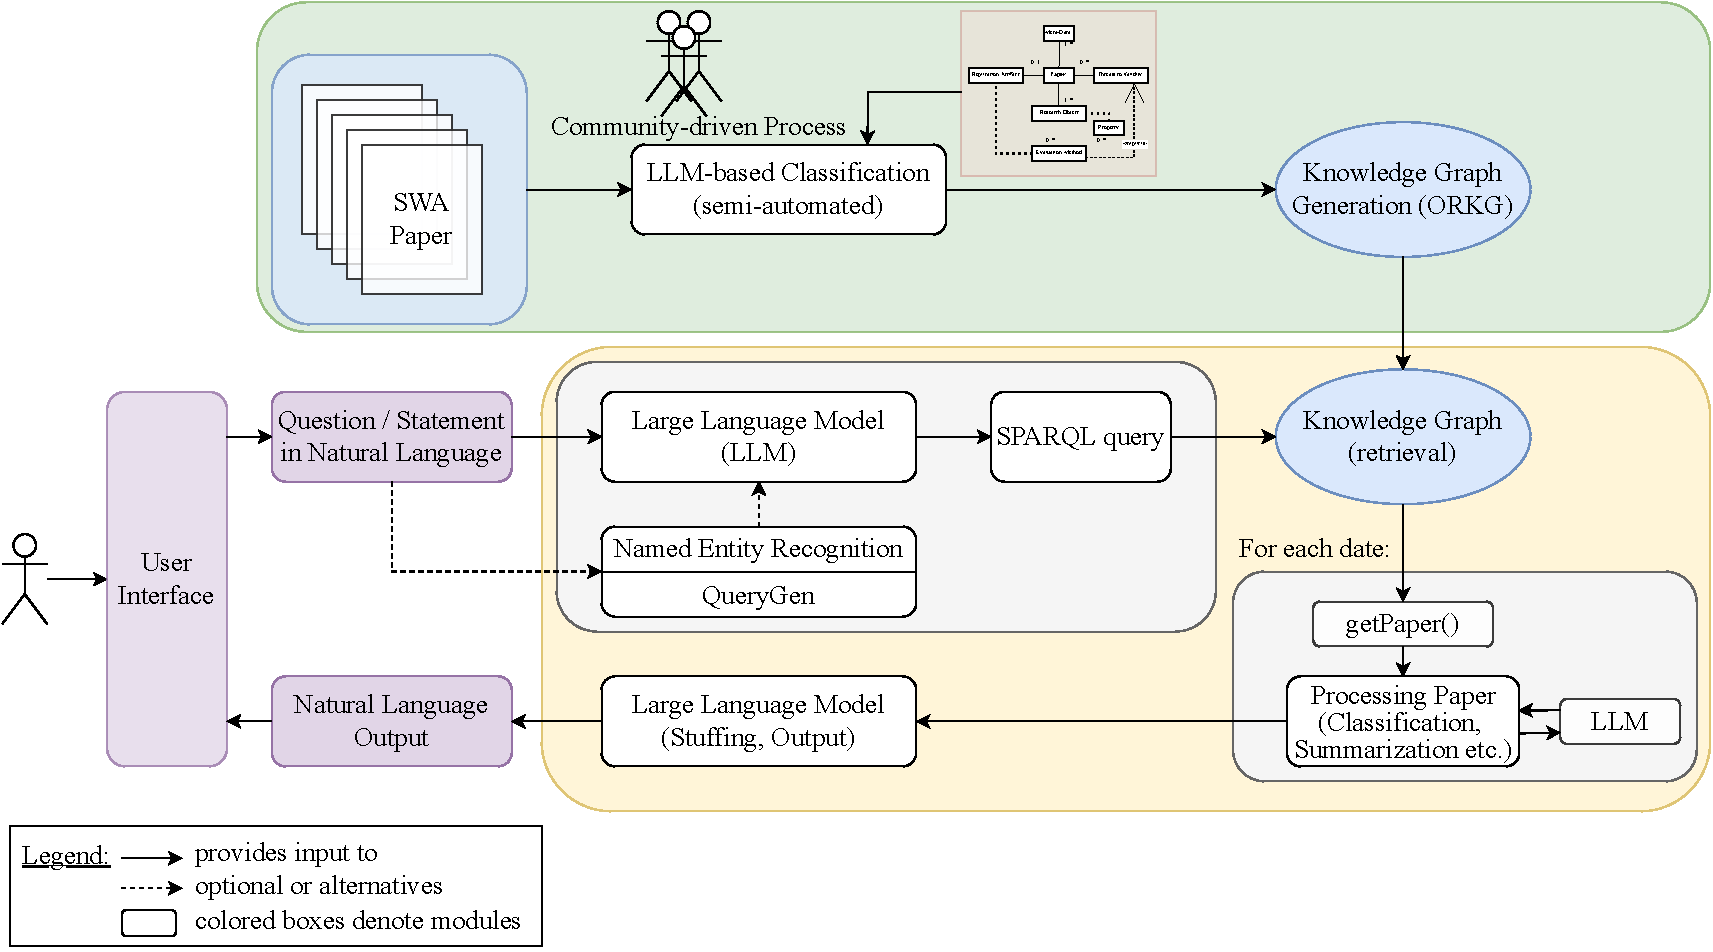
\includegraphics[width=0.95\textwidth]{figures/karagen.pdf}
    \caption[The KARAGEN Approach]{The KARAGEN approach, as proposed by \textcite{kaplan_combining_2024}, consists of two parts for a \gls{llm}-based retrieval on the \gls{orkg}. The green box shows the generation and population of the \gls{orkg}, while the yellow box depicts the \gls{llm}-based retrieval.}
    \label{fig:karagen}
\end{figure}

The \gls{karagen} approach is illustrated in \autoref{fig:karagen} and is composed of two parts: 1) Knowledge Graph Generation and Population and 2) Knowledge Retrieval. The following explanations are based on the descriptions provided by \textcite{kaplan_combining_2024}.

\paragraph{Knowledge Graph Generation and Population} This component is responsible for populating the \gls{orkg} with information through a semi-automated process, where users are supported by \gls{llm}-based classification. In the case of the \gls{orkg}, adding information about research papers is facilitated through templates. This means that either users or machines can fill in the required information into these templates, which are then stored in the graph as a contribution to the research paper.

\paragraph{Knowledge Retrieval} This component handles the retrieval and processing of knowledge from the graph. Users can submit queries in natural language, which are then processed using an \gls{llm}. The retrieval process may involve several steps, such as generating graph queries by matching natural language elements to graph components. Optionally, a knowledge enhancement component can be incorporated to transform and generate information. Finally, the system generates a response for the user. During this retrieval process, sources can be added to indicate the origin of the data and ensure traceability.

% In the following, we present the core concepts of the \gls{orkg}. This information is derived from \cite{ilangovan_open_2024} and the official \gls{orkg} website\footnote{\url{https://orkg.org/about} [last accessed on 21.12.2024]}.

% A recent study by \textcite{verma_scholarly_2023} reviewed 10 \glspl{rkg} that support scholarly infrastructures and found that nearly all used RDF for data representation. The study also highlighted that the core research-related entities across these graphs are quite similar, generally grouping into eight categories. The first group, \emph{People}, involves individuals such as authors and researchers. The second group, \emph{Publications}, relates to scholarly outputs like journal articles and conference papers. The third group, \emph{Organizations}, includes universities, research institutes, and other bodies that researchers belong to. The fourth group, \emph{Events}, covers academic gatherings like conferences and workshops. The fifth group, \emph{Datasets}, refers to digital collections or platforms where publications, data, and related resources are stored. The sixth group, \emph{Publishers \& Venues}, encompasses journals, conference venues, and other forms of publishers.

% TODO Add typical structure of a RKG \cite{verma_scholarly_2023}



% A \gls{kg} is an extended form of an ontology providing richer entity descriptions at the instance level \cite{ilangovan_open_2024}. 

% Mathematically speaking, a \gls{kg} stores structured knowledge as a collection of triples \(KG = \{(h,r,t) \subseteq \varepsilon \times R \times \varepsilon \} \), where \(\varepsilon\) denotes the entities and \(R\) the relation between the entities \cite{pan_unifying_2024}. These entities and their relationships are organized in a directed graph (\(G\)), defined as \(G = (V, E)\). In this graph, the vertices (\(V\)) correspond to the entities, and the edges (\(E\)) denote the relationships between them. Intuitively, a fact in the knowledge graph is formed by two entities connected by a relationship \cite{abu-salih_domain-specific_2021}.

% \Glspl{kg} have become an emerging technology in industry and in academia as they enable data to be organized \enquote{in a flexible, fine-grained, context-sensitive, and semantic representation to be understandable, processable, and usable by humans and machines \cite{karras_divide_2023}}.

% - A scholarly \gls{kg} is a type of graph that contains bibliographic information \cite{banerjee_dblp-quad_2023}. Some well known scholarly \glspl{kg} are the Microsoft Academic Graph, OpenAlex, ORKG, and DBLP.

% - The DBLP \gls{kg} includes bibliographic information on a wide range of topics within the field of computer science. It mainly consists of two entities \emph{Person} and \emph{Publication} \cite{banerjee_dblp-quad_2023}.  
% According to \textcite{taye_understanding_2010}, the semantic web aims to extend the current web by representing the information in both a human and machine-readable format. The backbone of the semantic web is formed by \emph{ontologies} by offering a shared conceptualization of a domain. An ontology consists of the following components:

% \begin{enumerate}
%     \item \emph{Concepts} are also referred to as classes or terms and represent abstract groups, sets, or collections of objects within a domain. They are organized hierarchically with parent and child relationships.
%     \item \emph{Instances} or individuals represent specific objects or elements of a concept.
%     \item \emph{Relations} or slots define how concepts are related to one another.
%     \item \emph{Axioms} are used to impose constraints on the values of concepts or instances. These are usually expressed in logic-based languages and ensure consistency within the ontology.
% \end{enumerate}

% \gls{rdf} is described as the first layer of the Semantic Web architecture \cite{taye_understanding_2010}. It provides the framework for representing metadata and semantics in a machine-readable format and can be applied to semi-formally describe ontologies. At the core of \gls{rdf} are triples, which are statements in the form of \((subject, predicate, object)\) \cite{wood_rdf_2014}. A \emph{subject} is the resource that is being defined, which can be either an \gls{iri} or a blank node. A \emph{predicate} is the property or relation between the subject and the object in the form of an \gls{iri}. The \emph{object} is the value or target of the relationship and can be either an \gls{iri}, a blank node, or a literal. A \gls{iri} acts as a unique identifier for resources, while literals are atomic pieces of information. Blank nodes are used to represent resources that do not have a unique identifier. 

% Combined as a set, triples form a \gls{rdf} graph which is a directed graph where the nodes represent entities and the edges represent the relationships between them \cite{hogan_knowledge_2022, paulheim_knowledge_2016, barrasa_building_2023}. When such a graph accumulates data to convey knowledge about the real world, making it comprehensible to both humans and machines, it is referred to as a \gls{kg}. 

\section{Knowledge Graph Question Answering (KGQA)}

\acrfull{kgqa} presents a research area that focuses on empowering users to access information stored within a \gls{kg} by formulating questions in natural language \cite{banerjee_knowledge_2024,chakraborty_introduction_2021,chakraborty_introduction_2019,pan_unifying_2024,yani_better_2022}. The primary objective of \gls{kgqa} is to retrieve answers from a \gls{kg} based on a question posed in natural language. This eliminates the necessity for users to write formal query languages such as SPARQL or possess intricate knowledge of the underlying structure and vocabulary of the \gls{kg} \cite{chakraborty_introduction_2021,chakraborty_introduction_2019,sabou_survey_2017}.

Historically, the research objective of enabling automated systems to answer questions posed in natural language precedes the modern adoption of \glspl{kg}. Early efforts in \acrfull{qa} explored systems designed to respond to questions by querying structured \acrfull{kb} or databases with early systems dating back to the 1970s and 1980s. A significant surge in interest in natural language question answering occurred with the establishment of a \gls{qa} track at the Text Retrieval Conferences (TREC), beginning in 1999. \cite{hirschman_natural_2001}

Due to advancements in semantic web technologies and automated information processing, the creation of large volumes of structured information became feasible \cite{chakraborty_introduction_2019}. \glspl{kg} emerged as a prime instance of storing structured data, which model facts about entities and their relationships, often in collections of triples \cite{chakraborty_introduction_2019,hogan_knowledge_2022,ji_survey_2022}. Consequently, \gls{kgqa} systems were developed to provide an intuitive natural language interface to query this structured knowledge contained in \glspl{kg}. Over time, several terms have been used for this task, including \acrfull{kbqa} \cite{ehrlinger_towards_2016} and \acrfull{sqa} \cite{sabou_survey_2017}. However, the term \gls{kb} has often been used misleadingly in the literature as a synonym for \glspl{kg} \cite{ehrlinger_towards_2016}.

 As \gls{kgqa} research progressed, the focus from simple questions requiring the retrieval of single facts shifted to more complex ones requiring multi-hop reasoning or constraints \cite{fu_survey_2020,banerjee_knowledge_2024,chakraborty_introduction_2021}. Two primary research directions emerged for building \gls{kgqa} systems: Methods based on \emph{\gls{ir}} gather question-related information from the \gls{kg} and leverage it to optimize the generation process. \emph{\gls{sp}-based methods} focus on the translation of the natural language question into a formal query or logical form that can be executed directly against the \gls{kg}.

 Neural networks became integral to various aspects of \gls{kgqa} systems across both \gls{ir} and \gls{sp} paradigms \cite{chakraborty_introduction_2019,ji_survey_2022}. Employed neural network architectures include embedding models, Recurrent Neural Networks (RNNs), Convolutional Neural Networks (CNNs), and Graph Neural Networks (GNNs) \cite{chakraborty_introduction_2021,pan_unifying_2024,ji_survey_2022}. More recently, the advent of pre-trained \glspl{llm} has begun to impact research on \gls{kgqa}. Although some research explores whether \glspl{llm} themselves can replace \glspl{kg}, most research is directed at the unification of \glspl{llm} and \glspl{kg} \cite{pan_unifying_2024}. In current research, \glspl{llm} are integrated into \gls{kgqa} systems in various ways. For instance, they can act as entity/relation extractors to extract data from questions, are used in \gls{sp} approaches to translate questions into formal queries, or are used in \gls{ir}-based approaches to function as reasoners over retrieved \gls{kg} subgraphs \cite{pan_unifying_2024}.


% Questions answered by KGQA systems are often divided into the categories—simple and complex. The questions, which can be answered by considering a single fact, without any additional constraints are generally defined as simple questions. For instance, the question “What is the birthplace of Michael Crichton” is a simple question since it can be answered by only considering the following fact: hex:Chicago, ex:birthPlaceOf, ex:Michael_Crichtoni. In contrast, the question “What is the birthplace of Westworld's writer?” is considered complex since answering this question requires knowing both hex:Michael_Crichton, ex:writerOf, ex:Westworldi and hex:Chicago, ex:birthPlaceOf, ex:Michael_Crichtoni. \cite{chakraborty_introduction_2021}

% In the QA community, KGQA is often also called knowledge base question answering (KBQA). \cite{chakraborty_introduction_2021}



% \acrfull{kgqa} is a relatively new research field with no established definition. In some works, \gls{kgqa} is used synonymously with \gls{kbqa} \cite{fu_survey_2020,peng_graph_2024}

\section{Large Language Models}
\label{sec:fundamentals_language_models}

\acrfullpl{llm} are pre-trained models with hundreds of billions of parameters generated by excessive training of very large corpora of text \cite{chung_scaling_2022}. These models are designed to estimate the probability distribution in a sequence of text, enabling them to perform a wide range of language-related tasks \cite{kojima_large_2023}. Recently, \glspl{llm} have demonstrated powerful capabilities in natural language understanding, expressiveness, general knowledge, and zero-shot generalization \cite{yang_give_2024}.

The architecture of most \glspl{llm} is derived from the \emph{Transformer} design, which includes encoder and decoder modules empowered by a self-attention mechanism \cite{pan_unifying_2024}. Based on their structure, \glspl{llm} can be broadly categorized into \emph{encoder-only}, \emph{decoder-only}, and \emph{encoder-decoder} models. Notable examples of these architectures are Flan T5 \cite{chung_scaling_2022} for the encoder-decoder framework, GPT-4 \cite{openai_gpt-4_2024} for the decoder-only framework, and DeBERTa \cite{he_deberta_2021} for the encoder-only framework. In this thesis, we focus on the decoder-only framework, as many state-of-the-art \glspl{llm} follow this architecture \cite{pan_unifying_2024}.

\subsection{Prompting} 
An important concept in leveraging \glspl{llm} is \emph{prompting}, which involves conditioning the model on a natural language instruction to guide its generation for desired tasks without any further training or gradient updates to its parameters \cite{wei_emergent_2022,kojima_large_2023}. Given this input prompt, the \gls{llm} then generates an answer in natural language. Popular prompting methods are \emph{few-shot prompting}, which involves adding a few examples \cite{brown_language_2020} or only adding instructions describing the task, which is referred to as \emph{zero-shot prompting} \cite{kojima_large_2023}. Another popular prompting method is Chain-of-Thought (CoT), where a chain-of-thought demonstration is provided during prompting \cite{wei_chain--thought_2023}. To maximize the effectiveness of \glspl{llm}, \emph{prompt engineering} is a new field that focuses on the creation and refinement of prompts \cite{pan_unifying_2024}.

\subsection{Limitations} 
Despite their impressive capabilities, \glspl{llm} face certain limitations. They are often described as black-box models, which means that they lack explainability and transparency, making it difficult for users to comprehend the reasoning behind their answers \cite{yang_give_2024,pan_unifying_2024}. Furthermore, \glspl{llm} are prone to generating factual errors or \emph{hallucinations} in which the \gls{llm} provides answers that contradict existing sources or lack evidence to support statements, which is particularly prominent when handling queries beyond their training data or when requiring current information \cite{gao_retrieval-augmented_2024,yang_give_2024}. Moreover, \glspl{llm} may not perform as well on domain-specific tasks as on general ones due to the limited availability of domain-specific corpus \cite{yang_give_2024}.

\subsection{Embedding Models}

A challenge concerning natural language processing is the representation of words and their associated meanings. One paradigm to approach this challenge is the use of vector representations in a continuous space. The fundamental idea behind these representations is that words that appear in similar contexts tend to have similar meanings. Consequently, within such a vector space, the proximity between word representations encodes semantic and syntactic regularities. These dense vectors are typically referred to as \emph{embeddings}. \cite{banerjee_knowledge_2024, pennington_glove_2014, mikolov_efficient_2013}

Early methods for learning representations of words, such as Word2Vec \cite{mikolov_efficient_2013} and GloVe \cite{pennington_glove_2014}, train word embeddings based on the co-occurrence statistics of words within a large text corpus. This class of embeddings is termed \emph{static} because the matrix produced during training is used without alteration. To address this limitation, \emph{dynamic} word embeddings utilize the advances of the transformer model to compute different representations for the same word depending on its context within the given sentence. Consequently, transformer-based pre-trained language models such as BERT \cite{devlin_bert_2019} have become relevant to solving the challenge of word representation. \cite{banerjee_knowledge_2024}


% \subsection{Graph Integration}
% Given these limitations and the complementary strengths of \glspl{kg} which explicitly store rich factual knowledge in a structured format, unifying \glspl{llm} and \glspl{kg} has become an active research direction \cite{pan_unifying_2024,peng_graph_2024}. Such a unification aims to leverage the advantages of both, enhancing the factual reasoning and interpretability of \gls{llm} answers while potentially using \glspl{llm} to aid in \gls{kg} construction and evolution \cite{pan_unifying_2024}.
 




% \subsection{Large Language Models}
% Research on PLMs has shown great success in scaling the model, which improves the capabilities of the model in downstream tasks, leading to surprising emerging abilities. Examples for such abilities that are not present in small models but arise in very large models are few-shot prompting, instruction following, and chain-of-thought \cite{wei_emergent_2022}.  

% Scaling PLMs to a certain threshold that emits these abilities is what distinguishes PLMs from \glspl{llm} \cite{yang_give_2024}. 

% This means that typically \glspl{llm} refer to PLMs that consist of hundreds of billions of parameters, with notable examples being: Flan T5 \cite{chung_scaling_2022} for the encoder-decoder framework, GPT-4 \cite{openai_gpt-4_2024} for the decoder-only framework, and DeBERTa \cite{he_deberta_2021} for the encoder-only framework. 

% 

% \subsection{Categorization}
% The architectural framework used in a PLM can be categorized into three types: encoder-only, decoder-only, and encoder-decoder \cite{wang_pre-trained_2023}. 

% \paragraph{Decoder-Only} 
% In the decoder-only approach, a unidirectional transformer decoder, operating from left to right, serves as the foundational mechanism during pre-training. This method employs an autoregressive technique for token prediction, in which each token is predicted based on its preceding tokens. Specifically, given a text sequence \(x = (x_1, x_2, x_3, ..., x_T)\), where \(x\) is the complete original sentence, \(x_t\) is the t-th token, and \(T\) is the total number of tokens, the model computes the probability of the sequence by the product \(p(x) = \prod^T_{t=1}p(x_t|x_{<t})\), representing the probability of each token given its previous sequence.

% \paragraph{Encoder-Only}
% Frameworks based on transformer encoders, such as the one used by BERT, employ bidirectional transformers to address the challenge of restoring altered tokens within sentences containing randomly masked elements. BERT exemplifies this approach through its use of a Masked Language Model (MLM) methodology, where specific tokens are substituted with a [MASK] token during the pre-training phase. The model then uses the surrounding contextual information to accurately predict the original tokens. Furthermore, BERT enhances its comprehension of text relationships by employing a Next Sentence Prediction (NSP) technique, which evaluates the links between consecutive sentences. This feature is beneficial for tasks that necessitate grasping sentence contexts, such as question answering.

% \paragraph{Encoder-Decoder}
% The encoder-decoder framework is tailored for training sequence-to-sequence (seq2seq) models. This process involves obscuring tokens within the source sequence and subsequently reconstructing them in the target sequence. Broadly, these frameworks are differentiated into two distinct types: 1) the seq2seq encoder-decoders, which integrate a bidirectional transformer encoder with a unidirectional transformer decoder, each posing independent parameters; and 2) the unified encoder-decoders, where both the bidirectional encoder and the unidirectional decoder are trained concurrently with the same set of parameters. This architecture is primarily devoted to tasks in natural language generation (NLG), as it equips the model to simultaneously manage tasks related to understanding and generating language.


\section{Graph Retrieval Augmented Generation (GraphRAG)}

 The paradigm of \acrfull{rag} has gained significant traction to mitigate issues with \glspl{llm}, such as hallucination, lack of domain-specific knowledge, and outdated information. The concept behind \gls{rag} is to improve the outputs of an \gls{llm} by providing it with relevant information retrieved from an external knowledge source at the time of inference instead of relying on the potentially outdated or imprecise knowledge internalized during pre-training. \cite{lewis_retrieval-augmented_2021,wu_retrieval-augmented_2024,peng_graph_2024,yang_give_2024}

A typical \gls{rag} system involves a \emph{retriever} component that obtains relevant information from a \gls{kb} and a \emph{generator} component that uses an \gls{llm} to generate a response based on the information retrieved and the question \cite{wu_retrieval-augmented_2024,yu_evaluation_2024}.

\acrfull{grag} represents an instantiation of the \gls{rag} paradigm where instead of retrieving information from unstructured text documents, \gls{grag} specifically targets and retrieves structured knowledge from graph databases such as \glspl{kg} or text-attributed graphs \cite{peng_graph_2024}. Consequently, \gls{grag} is positioned at the intersection of several key areas: traditional \gls{kgqa}, the \gls{rag} paradigm, and the emerging field of unifying \glspl{llm} and \glspl{kg} \cite{pan_unifying_2024,peng_graph_2024}.

A typical workflow of \gls{grag} comprises three main stages \cite{peng_graph_2024}:

\begin{enumerate}
    \item \textbf{Graph-based Indexing:} This constitutes the initial phase of \gls{grag}, where a pre-existing graph database is selected or constructed to then establish indices upon it to later facilitate efficient retrieval.
    \item \textbf{Graph-Guided Retrieval:} Given the provided input question, this phase aims to identify and extract a relevant subset of the graph data that is useful to provide an answer to the question.
    \item \textbf{Graph-Enhanced Generation:} In this final stage, the question and the retrieved graph knowledge are used as input for an \gls{llm} to produce the natural language response.
\end{enumerate}


% Authoren die RAG initial vorgestellt haben: \cite{lewis_retrieval-augmented_2021}
% Ein gutes Survey für RAG \cite{gao_retrieval-augmented_2024}
% Since the emergence of \glspl{llm}, a growing number of research has focused on \gls{rag} \cite{gao_retrieval-augmented_2024}.

% According to \textcite{yu_evaluation_2024} a typical \gls{rag} system comprises two main components: \emph{Retrieval} and \emph{Generation}. The purpose of the retrieval component is to extract information from \glspl{kb} that is relevant to a given query. There are two primary phases involved during retrieval: \emph{indexing} and \emph{searching}. 

% The searching phase is responsible for the retrieval of relevant information based on a given query. It can be categorized into three types: \emph{sparse retrieval}, \emph{dense retrieval}, and \emph{web search engine}. Sparse retrievers assess the similarity between the query and documents through weighted term matching and are not trained on specific data distributions. Typical methods are TF-IDF \cite{ramos_using_2003} and BM25 \cite{robertson_probabilistic_2009} which rely on keyword matching and word frequency. Although they excel at lexical matching, they do not recognize synonyms and paraphrases and therefore miss relevant context without keyword overlap. In contrast, dense retrievers evaluate similarity by employing representations learned from supervised QA datasets and leveraging pre-trained language models such as BERT \cite{he_deberta_2021} or GPT-4 \cite{openai_gpt-4_2024}. This capability enables them to identify relevant documents even with minimal keyword overlap, which is essential for complex queries that require contextual understanding. Lastly, retrieval over web search engine allows the retriever to traverse the extensive information in the web using search engines like Google Search\footnote{\url{https://developers.google.com/custom-search/v1/overview} [last accessed on 11.01.2025]} or Bing Search\footnote{\url{https://www.microsoft.com/en-us/bing/apis/bing-web-search-api} [last accessed on 11.01.2025]}. 

% Indexing is a preprocessing step that is performed before the search to organize information in a way that allows efficient retrieval. For sparse retrieval indexing involves the calculation of IDF for each term and storing the values in a database for a quick look-up and scoring when queried. Dense retrieval, on the other hand, encodes the information into dense vectors through the use of a pre-trained language model. The vectors are then indexed using a \gls{ann} search technique \cite{douze_faiss_2024}. For indexing large documents, the technique of chunking is frequently employed. It restricts similarity scores to specific segments instead of the entire text. This approach is particularly beneficial, as semantic embeddings tend to be less accurate for lengthy documents. Moreover, the information requested frequently tends to be brief in nature.

% The contexts retrieved during the search step are then used in the generation component of the \gls{rag} system to generate a final answer to the query. \textcite{yu_evaluation_2024} underscore the significance of prompting as a fundamental aspect upon which the generation process heavily relies. In the process of generation prompting, the query, relevant retrieval contexts, and instructions are combined into one comprehensive input for the \gls{llm} to utilize. The literature suggests various prompting techniques that may be employed to shape the output of the model. \gls{cot} encourages the model to generate a step-by-step reasoning process before arriving at a final answer \cite{wei_chain--thought_2023}. \gls{tot} extends the idea of \gls{cot} by exploring multiple lines of reasoning simultaneously, creating a tree of possible thought processes \cite{besta_graph_2024}. Self-Note involves the model to explicitly think and write down its thoughts \cite{lanchantin_learning_2023}. The \gls{rar} prompting strategy first rephrases and rewrites the user query before formulating a response \cite{deng_rephrase_2024}.

% In addition, after the generation of the final output, a post-processing step may be implemented where the output is formated according to the specific needs of the task or an expected output structure \cite{yu_evaluation_2024}.

% \subsection{Definition of GraphRAG}

% TODO: Transition from RAG to GRAPHRAG

% "From a broad perspective, GraphRAG can be seen as a branch of RAG, which retrieves relevant relational knowledge from graph databases instead of text corpus. However, compared to textbased RAG, GraphRAG takes into account the relationships between texts and incorporates the structural information as additional knowledge beyond text. Furthermore, during the construction of graph data, raw text data may undergo filtering and summarization processes, enhancing the refinement of information within the graph data." \cite{peng_graph_2024}

% \subsection{Categories of GraphRAG Approaches}
% \label{sec:categories_of_graphrag_approaches}

% \begin{table}[t]
%     \centering
%     \renewcommand{\arraystretch}{1.5}
%     \begin{tabular}{p{3cm}lp{4cm}p{4cm}}
%         \toprule
%         \textbf{Category} & \textbf{Type} & \textbf{Strengths} & \textbf{Weaknesses} \\ 
%         \midrule
%         \multirow{3}{*}{\textbf{Models}}         
%             & Non-parametric & Fast, low cost & Low accuracy \\ 
%             & LM-based & Accurate, handles natural queries & High computational cost\\ 
%             & GNN-based & Leverages graph structure & Complex to implement\\ 
%         \midrule
%         \multirow{3}{*}{\textbf{Paradigms}}      
%             & Once retrieval & Fast, low complexity & Limited scope \\ 
%             & Iterative retrieval & Adaptive, high accuracy & Longer runtime\\ 
%             & Multi-stage retrieval & Task-specific, modular & Requires careful design\\ 
%         \midrule
%         \multirow{4}{*}{\textbf{Granularity}}   
%             & Node-based & Targeted retrieval & Lacks relational context\\ 
%             & Triplet-based & Handles relationships & Limited to triple scope\\ 
%             & Path-based & Captures sequences & High computational load\\ 
%             & Subgraph-based & Comprehensive retrieval & Complex and costly\\
%         \midrule
%         \multirow{2}{*}{\textbf{Training Strategy}}   
%             & Training-Free & Avoiding high training costs & Careful prompt engineering \\ 
%             & Training-Based & Adaptive to specific tasks & Requires costly training\\ 
%         \midrule
%         \multirow{2}{*}{\textbf{Indexing}}   
%             & Graph Indexing & Preserves graph structure & Long retrieval times \\
%             & Text Indexing & Simple textual content retrieval & Limited to text-based queries\\
%             & Vector Indexing & Quick and efficient search & Requires vectorization \\
%             & Hybrid Indexing & Combines advantages of other methods & Complex to implement \\
%         \bottomrule
%     \end{tabular}
%     \caption{Comparison of GraphRAG categories according to \cite{peng_graph_2024}}
%     \label{tab:retrieval_comparison}
% \end{table}

% To better understand the landscape of \gls{grag} approaches proposed by the literature, researchers have proposed different taxonomies to categorize these approaches. In this section, we examine two prominent taxonomies: one proposed by \textcite{peng_graph_2024} that focuses on technical aspects like models and retrieval strategies, and another by \textcite{pan_unifying_2024} that emphasizes the integration between \glspl{llm} and \glspl{kg}.

% \textcite{peng_graph_2024} propose to categorize the approaches based on the underlying \emph{Model}, \emph{Retrieval Paradigm}, \emph{Retrieval Granularity}, \emph{Training Strategy}, and \emph{Indexing}. Table \ref{tab:retrieval_comparison} provides an overview of the categories, highlighting the strengths and weaknesses of each category.

% \paragraph{Model Categorization} Retrievers can be categorized into three types, based on their underlying models. The \emph{Non-parametric} retriever type is based on heuristic rules or traditional graph search algorithms. They often include a linking pre-processing step to identify nodes in the graph before the retrieval. Because these methods are not using deep-learning models, they are able to achieve fast retrieval times with low costs. However, they suffer from inaccurate retrieval. The \emph{LM-based} retriever, on the other hand, shows strong performance in processing and interpreting diverse natural language queries. They are based on pre-trained language models like GPT-4 \cite{openai_gpt-4_2024}, and can be further categorized into two types: discriminative and generative. The discriminative models focus on estimating the conditional probability and are effective in task such as text classification and sentiment analysis. Discriminative models, on the other hand, show great potential in language understanding and in-context learning. While LM-based retrievers offer a higher retrieval accuracy, they require significantly more computational overhead compared to the Non-parametric retrievers. The third type, the \emph{GNN-based} retriever, utilizes a GNN model to understand and leverage complex graph structure. They typically encode the graph data and subsequently score different retrieval granularities based on their similarity to the query.

% \paragraph{Retrieval Paradigm} Additionally, GraphRAG retrievers can be categorized based on the retrieval paradigm they employ. This categorization classifies retrievers according to how frequently they access information in the graph and whether there are phases during which the information is processed. There are three paradigms: once retrieval, iterative retrieval, and multi-stage retrieval.
% \emph{Once retrieval} refers to retrievers that access the graph with only a single query to obtain all the information required for the retrieval process. Examples of this approach include embedding-based methods or those that use predefined rules or patterns to formulate queries to the graph. The once retrieval paradigm is typically faster as it involves lower complexity.
% \emph{Iterative retrieval}, on the other hand, refers to retrievers that access the graph multiple times to gather the information needed for the retrieval process. Here, several retrieval steps are executed sequentially, with each subsequent step depending on the results of the previous retrieval step. This approach can be either adaptive, for instance, when models autonomously decide which steps to execute next and when to terminate the retrieval process, or non-adaptive when the steps are predetermined and termination is based on predefined parameters. The iterative paradigm generally has longer runtimes, especially when \glspl{llm} are used, but offers higher accuracy.
% Lastly, there is the \emph{multi-stage retrieval} paradigm. In this paradigm, the retrieval process is divided into multiple phases, each with a different task. For example, different retrieval methods can be used in different phases, or generation processes can be integrated into the retrieval process.

% \paragraph{Retrieval Granularity} Furthermore, retrievers can be categorized based on the retrieval granularity they use. The retrieval granularity refers to the level of detail at which the retriever retrieves information from the graph. There are four types of granularities proposed by \textcite{peng_graph_2024}: Nodes, Triplets, Paths, and Subgraphs. \emph{Node-based retrievers} retrieve information at the node level, which means that they retrieve information from individual elements in the graph. This is ideal for targeted queries where specific information from the graph should be extracted. \emph{Triplet-based retrievers} retrieve information at the triplet level, which consists of both the nodes and their relationships in the form of subject-predicate-object tuples. This granularity is useful for queries that require information about the relationships between nodes, for example, when contextual relevance between entities is required. When sequences of relationships between entities are required, \emph{Path-based retrievers} are used. However, for comprehensive relational contexts within a graph, a \emph{Subgraph-based retriever} might be required. 

% \paragraph{Training Strategy} In the classification of retrievers based on their training strategy, a distinction is made between Training-Free and Training-Based Retrievers. \emph{Training-Free Retrievers} are retrievers that do not require a training phase and can be applied directly to the graph. Retrievers of this category often rely on carefully defined prompts, as \glspl{llm} like GPT-4 \cite{openai_gpt-4_2024} are frequently used. There are several sub-categories of Training-Free Retrievers. Non-parametric retrievers operate with predefined rules or traditional graph search algorithms and do not use specialized models. On the other hand, there are retrievers that work with pre-trained \glspl{llm}. For example, pre-trained embedding models are used, which are applied to the graph in an indexing step. Additionally, there are approaches that send graph elements such as entities, triples, paths, or subgraphs as part of a prompt to an \gls{llm} to obtain a selection or answer. \emph{Training-Based Retrievers}, on the contrary, require a training or fine-tuning phase in which supervised signals are used. However, these variants are often challenging because they require ground truth data, which is frequently unavailable.

% \paragraph{Indexing} The retrieval approaches can also be categorized based on the indexing strategy they use. There are four types of indexing strategies: Graph Indexing, Text Indexing, Vector Indexing, and Hybrid Indexing. \emph{Graph Indexing} preserves the entire structure of the graph. It is often seen in conjunction with classic graph search algorithms such as BFS and Shortest Path algorithms. \emph{Text Indexing} involves to convert the graph structures to textual representations which are then stored in a corpus. Various sparse and dense retrieval techniques are applied to retrieve the relevant information. \emph{Vector Indexing} directly transforms the structures of the graph into vectors which are then stored in a database. Finally, \emph{Hybrid Indexing} is a combination of the three indexing strategies mentioned above.

% Another taxonomy is proposed by \textcite{pan_unifying_2024}. They focus on the unification of \glspl{llm} with \glspl{kg} to synergize the advantages of both technologies. The taxonomy includes various tasks such as incorporating the \glspl{kg} into the \gls{llm} during pre-training, fine-tuning, and inference. They also consider to use the \gls{llm} to improve the \gls{kg} by enriching the graph representation. In the following we are going to look at the proposed categories for retrieval in a \gls{qa} setting.

% \paragraph{KG-enhanced LLM inference} categorizes research that uses \glspl{kg} during the inference stage of \glspl{llm}. These methods do not require to retrain the model as they add up-to-date information to the \gls{llm} at inference time. A popular method to inject this knowledge is articulated by the authors as \emph{Retrieval-Augmented Knowledge Fusion}. Here, relevant knowledge is retrieved from a large corpus and then fused into the \gls{llm} during inference. Another method is \emph{KGs Prompting}. Here, the structure of the \gls{kg} is added to the prompt during inference to guide the \gls{llm} in generating the answer. The challenge in this category is to carefully design a prompt that converts the structured graph information into text sequences that the \gls{llm} can understand. 

% \paragraph{LLM-augmented KG Embedding} focuses on methods that map each entity and relation into a low-dimensional vector space. By applying this approach, the embeddings contain both the semantic kownloedge and structural information of the \gls{kg}. These embeddings are then used in tasks such as \gls{qa}, reasoning, and recommendation. There are two subcategories in this category: \emph{LLMs as Text Encoders} and \emph{LLMs for Joint Text and KG Embedding}. The former uses a embedding model to encode the textual information of the \gls{kg} into embeddings, while the latter directly encodes both the textual information and the graph structure into embeddings by training the \gls{llm}.

% \paragraph{LLM-augmented KG Question Answering} has the aim to provide answers to natural language questions based on the facts that are stored in the \gls{kg}. There are two subcategories in this category: First \emph{LLMs as Entity/Relation Extractors} has the goal to identify and extract entities and relationships that are mentioned in the natural language question to then retrieve relevant facts from the \gls{kg} based on this extraction. The second subcategory is \emph{LLMs as Answer Reasoners}. In this category, the facts are already retrieved from the graph and the goal is to reason over these facts to generate the answer to the question.

% \paragraph{Synergized Reasoning} includes methods that design synergized models capable of leveraging both the representational power of \glspl{llm} and the structured, relational knowledge of \glspl{kg} to perform complex reasoning. Notably, synergized reasoning often uses carefully designed architectures or joint training objectives to balance the benefits of continuous text-based representations with the discrete relational structures from \glspl{kg}. There are two subcategories in this category: First, \emph{LLM-KG Fusion Reasoning} adopts end-to-end trained \gls{llm} and \gls{kg} encoders to represent the knowledge in a unified space. Then a synergized reasoning module is applied to jointly infer answers. Second, \emph{LLMs as Agents Reasoning} employ the \gls{llm} itself as an active agent to retrieve and reason over graph-based knowledge without requiring additional training costs.



% To be able to find answers to a given question in a \gls{kg}, the user needs to have a in-depth understanding of the structure of the graph and its query language \cite{tran_comparative_2022}. To ease the access to information in a \gls{kg}, a significant effort has been put into building \gls{qa} systems that allow users to express their questions in natural language and for the system to find the relevant information for the user \cite{tran_comparative_2022}\cite{pang_survey_2022}\cite{bouziane_question_2015}\cite{thambi_towards_2022}\cite{liu_question_2015}.

% A \gls{kg} retriever refers to a methodology that retrieves relevant information from a \gls{kg}. Information is relevant, when it helps to answer a given question. 
% TODO: Add a bit of history to how the retrieval evolved
% mathematiccaly describe the problem: https://arxiv.org/pdf/2202.13296

% Warum gerade "LLMs to guide the retreival process". Vor- und Nachteile? Welche Alternativen gibt es hier noch das umzusetzen?
% In the context of this thesis, we refer to retrievers that retrieve information from a \gls{kg} based on a specified question while using a\gls{llm} to guide the retrieval process, as \gls{kglmqa} retrievers.
% TODO: Ausformulieren


% \begin{definition}[Topic Entity]
% \label{def:topic_entity}
% \leftskip=2em
%     The Topic Entity refers to an entity within the graph that serves as the starting node for the retrieval process. The retriever begins its traversal from this entity to locate relevant information corresponding to a specific query.
% \end{definition}

% \subsection{Multi-Hop Retrieval issue}

% Queries that require the retriever to reason and retrieve multiple contexts from the \gls{kb} is referred to as \emph{multi-hop} retrieval. This differs from single-hop queries where the answer can be directly derived from a single piece of context \cite{tang_multihop-rag_2024}. 

% Due to the multifaceted nature of such queries, multi-hop retrieval is a challenging task as traditional similarity matching methods like cosine similarity might not yield optimal results \cite{tang_multihop-rag_2024}.



% As shown in the study by \textcite{yu_decaf_2023}, current \gls{llm} based retrievers on \glspl{kg} struggle with multi-fact retrieval. 

\section{Approximate Nearest Neighbor (ANN) Search}
\label{sec:fundamentals_ann_search}

\acrfull{ann} search is a technique used to find data points that are likely close or similar to a given query point in a high-dimensional vector space. Unlike \gls{enn} search, which guarantees finding the absolute closest data points, \gls{ann} search trades some accuracy for significantly improved efficiency and speed \cite{douze_faiss_2024,wu_retrieval-augmented_2024}. The core idea behind \gls{ann} search is to preprocess the data into an indexing structure that tries to achieve a trade-off between search quality and search efficiency \cite{wu_retrieval-augmented_2024}. 
% Techniques include choosing appropriate distance metrics and advanced \gls{ann} indexing algorithms.

To understand the value of \gls{ann} search, it is helpful to first consider \gls{enn} search. Given a dataset of vectors ${x_i, i=1..N} \subset \mathbb{R}^d$ and a query vector $q \in \mathbb{R}^d$, a typical \gls{enn} search involves finding the index $n$ of the database vector $x_n$ that minimizes the distance to $q$, typically using a distance metric such as the Euclidean Distance (L2). Other popular similarity metrics are cosine similarity or inner product similarity, for which the objective would be to maximize the score. \cite{douze_faiss_2024}

A straightforward technique for \gls{enn} search is brute force, which involves calculating the distance between the query vector $q$ and every single database vector $x_i$ and then identifying one or more vectors with the smallest distance. The amount of vectors is often denoted by a $k$ parameter. However, this process is slow on large datasets where \gls{ann} search comes in handy. Here, database vectors are preprocessed in a specialized indexing structure to allow for quickly narrowing down the search space at query time. \cite{douze_faiss_2024,wu_retrieval-augmented_2024}

Various different \gls{ann} indexing techniques exist. \emph{Inverted File System with Product Quantization (IVFPQ)} involves the partitioning of the vector space by applying clustering algorithms to then use fine-grained quantization to compress the vectors. \emph{The Hierarchical Navigable Small World (HNSW)} is a technique that builds hierarchical graph structures where each node represents a vector. \emph{Tree-based Indexing} organizes the vectors into hierarchical tree-like structures to separate the vector space. \cite{wu_retrieval-augmented_2024}



% The accuracy of ANNS is typically measured as a discrepancy with exact search results. For k-nearest neighbour search, a common metric is "n-recall@k," which is the fraction of the true n nearest neighbors found within the k first search results. \cite{douze_faiss_2024}



\section{Evaluation Metrics}
\label{sec:fundamentals_evaluation_rag}

To evaluate \gls{grag} approaches, the evaluation metrics can be broadly categorized into two types: \emph{generation} and \emph{retrieval} quality \cite{peng_graph_2024,yu_evaluation_2024}. Evaluating the generation quality is about the assessment of the generated answer, while the retrieval quality is about the of retrieved information and the coverage of the answer.


\subsection{Evaluating the Retrieval Component}

The evaluation of retrievers dates back to early information retrieval research. Conventional metrics typically compare the retrieved contexts with a set of \emph{golden-labeled} contexts. These metrics fall into two types: \emph{Rank-agnostic} or \emph{Rank-aware}, depending on whether they consider the order in which the contexts are retrieved \cite{yu_evaluation_2024,alinejad_evaluating_2024}. In the following, we introduce commonly used metrics based on  \textcite{yu_evaluation_2024, ibrahim_survey_2024,hu_unveiling_2024}.

\paragraph{Rank-agnostic Metrics} These metrics measure the quality of retrieval without considering the position of the item in the list of retrieved contexts. 

\begin{itemize}
    \item \textbf{Accuracy:} An assessment of the ratio of correctly retrieved contexts compared to the total number of retrieved contexts.
    
    \[
    \text{Accuracy} = \frac{TP + TN}{TP + TN + FP + FN}
    \]

    \gls{tp} refers to contexts that are relevant to the query and are accurately retrieved. \gls{tn} refers to contexts that are irrelevant to the query and have not been retrieved. \gls{fp} refers to contexts that are irrelevant to the query but have been incorrectly retrieved. \gls{fn} refers to contexts that are relevant to the query but have not been retrieved.

    \item \textbf{Precision:} Measures the proportion of relevant contexts retrieved by the system to the total number of contexts retrieved by the system.
    
    \[
    \text{Precision} = \frac{TP}{TP + FP}
    \]

    \item \textbf{Recall:} Quantifies the proportion of relevant contexts that have been retrieved from the total number of relevant contexts for a given query, considering the top \(k\) results.
    
    \[
    \text{Recall} = \frac{TP}{TP + FN}
    \]

    \item \textbf{F1:} An assessment which calculates the harmonic mean of precision and recall.

    \[
    \text{F1} = 2 \times \frac{Precision \times Recall}{Precision + Recall}
    \]
\end{itemize}


\paragraph{Rank-aware Metrics} These metrics additionally evaluate the order in which relevant items are presented. Typically, the higher the relevant item is placed in the list, the better the score.

\begin{itemize}
    \item \textbf{Hits@k} A measure of the fraction of correct retrieved contexts that appear in the top \(k\) total of retrieved contexts.
    \[
    \text{Hits@k} = \frac{H_k}{N_{query}}.
    \]
    In the above formula, \( H_k \) is the number of times a relevant context entry is in the top-k and \(N_{query}\) is the total amount of retrieved context.

    \item \textbf{Mean Reciprocal Rank (MRR)} Measures the average of the inverse ranks of the first relevant context retrieved by the system. This means that the metric focuses on how high the retriever ranks the first relevant context.
    \[
    MRR = \frac{1}{|Q|} \sum^{|Q|}_{i=1} \frac{1}{rank_i}
    \]
    In the formula given above, \(|Q|\) represents the total number of queries, and \(rank_i\) denotes the rank position of the first relevant document for the \(i\)-th query.
    
    \item \textbf{Mean Average Precision (MAP)} Computes the average of the precision values at different cut-off points for each query. Consequently, this metric gives an aggregate view on how well the retriever ranks the relevant contexts.
    \[
    MAP =  \frac{1}{|Q|} \sum^{|Q|}_{q=1} \frac{\sum^n_{k=1} (P(k) \times rel(k))}{|relevant \space documents_q|} 
    \]
    In the formula given above, \(P(k)\) represents the precision at position \(k\) in the ranking list, and \(rel(k)\) is an indicator function that is one if the document at rank \(k\) is relevant and zero otherwise. In addition, \(n\) denotes the total number of documents retrieved.

    \item \textbf{Exact Match (EM)} quantifies the proportion of retrieved contexts that exactly match the expected contexts.
    \[
    Exact Match = \frac{PEM}{N_{pred}}
    \]
    Where in the formula \(PEM\) is the proportion of the exact matches and \((N_{pred}\) is the total number of expected contexts.
\end{itemize}


\subsection{Evaluating the Generation Component}

To assess the quality of the generated answer, often traditional metrics are borrowed from other natural language processing tasks like machine translation or summarization \textcite{yu_evaluation_2024,ibrahim_survey_2024,alinejad_evaluating_2024,alinejad_evaluating_2024}. However, these metrics often fail to fully capture the performance within an \gls{llm}-based \gls{qa} system \cite{alinejad_evaluating_2024}. Consequently, \gls{llm} models are employed as evaluative judges to assess the quality of generated answers \cite{es_ragas_2023}.

\paragraph{Traditional Natural Language Processing Generation Metrics} Common metrics that are applied to the evaluation in \gls{rag} are \textcite{yu_evaluation_2024,ibrahim_survey_2024,alinejad_evaluating_2024,alinejad_evaluating_2024}:

\begin{itemize}
    \item \textbf{ROUGE} \gls{rouge} is a set of metrics that evaluate the quality of the generated text by comparing it to the ground truth. There are multiple variants available: \gls{rouge}-N calculates recall by comparing the presence of n-grams in the generated text and the ground truth. \gls{rouge}-L uses the longest common subsequence to capture meaning in the generated text. \gls{rouge}-W additionally uses weights for consecutive matches, distinguishing between spatially aligned and scattered matches. \gls{rouge}-S incorporates skip-bigrams to balance flexibility and structure sensitivity. \gls{rouge}-SU is a variant of \gls{rouge}-S that uses skip-bigrams and unigrams to evaluate the quality of the generated text \cite{lin_rouge_2004}.

    \item \textbf{BLEU} The \acrfull{bleu} metric measures the quality of the generated text by comparing it with the ground truth by calculating the overlap of n-grams\cite{papineni_bleu_2001}. The \gls{bleu} score is calculated as:
    \[
    BLEU = BP \cdot \exp\left(\sum^N_{n=1} w_n \log p_n\right)
    \]
    In this formula, \(BP\) is the brevity penalty that penalizes short-generated translations, \(w_n\) is the weight for the n-gram, and \(p_n\) is the precision of the n-grams that match the reference.

    \item \textbf{BertScore} This metric uses contextual embeddings that, unlike n-gram-based metrics, capture the semantic meaning of the generated text. BertScore uses pre-trained transformer models like Bert to transform the generated text and the ground truth into embeddings. With the embeddings, the cosine similarity between the generated text and the ground truth is calculated, resulting in precision, recall, and f1 scores \cite{zhang_bertscore_2020}

\end{itemize}

\paragraph{LLM as a Judge Metrics} \glspl{llm} can be prompted with an evaluation scheme to assess the answers based on user-defined metrics. They have shown a great ability to capture semantic nuances and attend to variations in answers \cite{alinejad_evaluating_2024,yu_evaluation_2024}. Recently, a framework has been established focused on providing different \gls{llm}-based metrics \cite{es_ragas_2023}. Their framework is available online\footnote{\url{https://github.com/explodinggradients/ragas} [last accessed on 26.03.2025]} from which the following metric explanations have been taken from:

\begin{itemize}
    \item \textbf{Faithfulness} Measures the factual consistency of the generated answer against the given context, where the answer is regarded as faithful if all the claims made by the answer can be inferred from the given context.
    \[
    \text{Faithfulness} = \frac{\text{Number of supported claims}}{\text{Total number of claims}}
    \]

    \item \textbf{Answer Relevancy} Focuses on how relevant the answer is to the question where higher scores indicate better alignment while lower scores are given if the answer is incomplete or includes redundant information. To calculate the score, an \gls{llm} generates $N$ questions based on the generated answer and then calculates the cosine similarity between the actual question and the generated questions.
    \[
    \text{Answer Relevancy} = \frac{1}{N}\sum^N_{i=1}\text{cosine similarity}(E_{g_i},E_o)
    \]
    Where $N$ denotes the number of generated questions, $E_{g_i}$ the embedding of the i-th generated question, and $E_o$ is the embedding of the actual question.

    \item \textbf{Factual Correctness} evaluates how well the generated answer aligns with a golden reference. The \gls{llm} decomposes both answers into individual claims and computes \gls{tp}, \gls{fp}, and \gls{fn} as follows:
    \[
    \begin{aligned}
    \text{True Positives (TP)} &= \text{Claims in the answer also found in the reference} \\
    \text{False Positives (FP)} &= \text{Claims in the answer not found in the reference} \\
    \text{False Negatives (FN)} &= \text{Claims in the reference not found in the answer}
    \end{aligned}
    \]
    Precision, recall, and F1 scores are then calculated using these values, as defined above.
\end{itemize}


\subsection{Micro vs. Macro Averaging}
When evaluating the performance of systems across a dataset of multiple questions, the overall performance needs to be assessed through aggregation. There exist two common types of aggregate scores: \emph{micro-averaging} and \emph{macro-averaging} \cite{hu_unveiling_2024}:

\begin{enumerate}
    \item \textbf{Micro-Averaging} calculates the aggregation of metrics globally, for example, by counting the overall \gls{tp}, \gls{fn}, \gls{tn}, and \gls{fp} scores to calculate micro-Precision, micro-Recall, and micro-F1. This approach gives equal weight to each individual retrieved-context across all questions. Consequently, questions that involve a larger number of such individual contexts will have a proportionally greater influence on the overall micro-averaged score.
    
    \item \textbf{Macro-Averaging} calculates each metric independently for each question and then takes the unweighted mean of the resulting scores. This essentially gives equal weight to each question, regardless of the number of contexts requested. It prevents the metric from being skewed by the performance of majority classes and ensures that the performance of minority classes is also represented.
\end{enumerate}

The choice of the preferred averaging method depends on the evaluation goals. In \gls{llm}-based evaluations, \emph{macro-averaging} is the preferred metric as observed by \textcite{hu_unveiling_2024}. The authors suggest that this calculation is preferred as it ensures that all classes, regardless of size, are considered equally.


\subsection{Sustainability Metrics}

\textcite{kaplan_responsible_2025} highlight the importance of integrating sustainability metrics into the evaluation of natural language processing systems. They advocate for assessments that consider both performance and environmental aspects by tracking the energy consumption measured in kilowatt-hours (kWh) or megajoules (MJ) and the carbon emissions in CO$_2$. The authors propose several metrics for evaluating sustainability either by using energy consumption or carbon emissions:


\begin{itemize}
    \item \textbf{Total Carbon Emission (CE):} Represents the absolute carbon footprint, measured in kilograms of CO$_2$ equivalents (kg CO$_2$e), resulting from the operation of the system during training or inference.

    \item \textbf{Relative Carbon Emission (CE$_rel$):} Links environmental impact directly to performance metrics, facilitating the assessment of carbon efficiency per unit of performance. The performance metric should be chosen based on the context.
    \[
    \text{CE}_{rel} = \frac{\text{CE}}{\text{Performance Metric}}
    \]

    \item \textbf{Delta-based Carbon Emission ($\Delta$CE):} To compare different systems performance improvements against carbon emissions. Using the lowest-performing system as a baseline, this metric reveals the environmental cost-effectiveness between two systems:
    \[
    \Delta\text{CE} = (\text{Performance Metric} - \text{Performance Metric}_{base}) \times \frac{\text{CE}_{base}}{\text{CE}}
    \]

    \item \textbf{Normalized Carbon Emission (nCE and nCE\textsubscript{rel}):} Normalizes the carbon emissions between the best and worst performing systems, providing a standardized scale (0 to 1) for easier comparison across different evaluations:
    \[
    n(\text{CE}) = 1 - \frac{\text{CE} - \text{CE}_{lowest}}{\text{CE}_{highest} - \text{CE}_{lowest}}
    \]
    \[
    n(\text{CE}_{rel}) = 1 - \frac{\text{CE}_{rel} - \text{CE}_{rel,lowest}}{\text{CE}_{rel,highest} - \text{CE}_{rel,lowest}}
    \]
\end{itemize}






% evaluates the broader societal and environmental impact of a system. Metrics focus on minimizing resource use, ensuring technical durability, and aligning the development with ethical and societal goals \cite{becker_sustainability_2015}.
% \textcite{kaplan_responsible_2025}


% However, traditional methods focus on retrieval that has a high top k recall, rather than taking into account that useful information has been recovered \cite{yu_evaluation_2024}. For this reason, new methods, known as llm-as-a-judge, have become a standard practice in which an \gls{llm} is used to evaluate semantic information between retrieved contexts and the ground truth \cite{alinejad_evaluating_2024,yu_evaluation_2024,salemi_evaluating_2024}.

% \paragraph{RAGAS} is a framework that employs various metrics that use \glspl{llm} to evaluate the generation and retrieval component of a \gls{rag} system. Since the publication of the framework in \cite{es_ragas_2023}, the set of available metrics has been updated\footnote{\url{https://docs.ragas.io/en/latest/concepts/metrics/available_metrics/} [last accessed on 14.01.2025]}. RAGAS provides \emph{Context Precision} to evaluate for each retrieved context whether the context is relevant or not using an \gls{llm}. Furthermore, \emph{Context Recall} divides the golden answer into claims to check if each claim is included in the context.

% For the evaluation of the generated answer it is still common to use traditional metrics like \gls{rouge} and \gls{bleu} that do not require the use of a language model. However, it is becoming standard to include language models as evaluative judges to be able to capture the context of the generated answer \cite{yu_evaluation_2024}.

% \paragraph{RAGAS} is a framework that provides a comprehensive list of metrics both \gls{llm}-based and non-\gls{llm}-based to evaluate the quality of the generated text. These include \emph{Faithfulness} to quantify whether the generated answer is grounded in the retrieved context and \emph{Answer Relevance} to evaluate if the generated answer appropriately addresses the user query \cite{es_ragas_2023}. 

\section{Taxonomies}
\label{sec:fundamentals_taxonomy}

A taxonomy is understood as a classification system designed to organize objects or concepts \cite{kundisch_update_2022,usman_taxonomies_2017,nickerson_method_2013,kaplan_introducing_2022}. Although terms such as \emph{classification}, \emph{framework}, and \emph{typology} are sometimes used interchangeably, the term \emph{taxonomy} is used most frequently in the literature \cite{nickerson_method_2013}. Consequently, for the remainder of this thesis, we will also use the term taxonomy.

Historically, taxonomies have been fundamental to research and practices across numerous disciplines, including natural sciences, social sciences, organizational science, strategic management, and information systems, as they are essential systems for structuring and understanding complex bodies of knowledge \cite{nickerson_method_2013,kundisch_update_2022}. The essence of a taxonomy is the classification process, a crucial cognitive task integral to conceptualization, language, mathematics, statistics, and overall data analysis \cite[7,11]{bailey_typologies_2003}. A \emph{classification} is described as a process or system of organizing objects into groups or classes based on their similarity \cite{nickerson_method_2013}.

\subsection{Formal Definition}
Formally, a taxonomy $T$ can be understood as a set of $n$ dimensions $D_i(i=1, \dots,n)$, where each dimension consists of $k_i \geq2$ characteristics $C_{ij}(j=1,\dots k_i)$ such that for any object of interest a classification based on $C_{ij}$ for each $D_i$ can be applied \cite{nickerson_method_2013}. Although some taxonomies require the classification of each dimension to be mutually exclusive, we consider this not to be a mandatory characteristic.


\subsection{Approaches to Taxonomy Development}

Historically, the methodologies utilized in the creation of taxonomies have traditionally been classified into two primary categories \cite{bailey_typologies_2003,nickerson_method_2013}:

\begin{itemize}
    \item \textbf{Conceptual (Deductive):} In this method, the researcher suggests categories or types derived from established theories, concepts, or models, typically without depending on empirical data, though such data may be employed for validation purposes. 
    \item \textbf{Empirical (Inductive):} Here, the process begins with empirical data about objects, and the classification is derived from this data, frequently using statistical techniques like cluster analysis.
    \item \textbf{Hybrid:} This approach combines conceptual and empirical elements and allows taxonomy developers to move back and forth between theoretical conceptualization and empirical observation.
\end{itemize}

However, often there is no systematic approach used for the creation of a taxonomy as it is created ad-hoc on the basis of intuition \cite{nickerson_method_2013,usman_taxonomies_2017,kundisch_update_2022}. To provide researchers with a systematic framework that helps in the creation of taxonomies, several approaches have been defined in the literature \cite{nickerson_method_2013,usman_taxonomies_2017,kundisch_update_2022,bayona-ore_critical_2014}. One such approach has been proposed by \textcite{usman_taxonomies_2017}, which is based on the taxonomy construction process from \textcite{bayona-ore_critical_2014}. This process involves five phases:

\begin{enumerate}
    \item \textbf{Planning} Is about defining the context and initial setting of the taxonomy.
    
    \item \textbf{Identification and Extraction} Is about the identification of terms that are relevant for the taxonomy with its subsequent extraction.

    \item \textbf{Design and Construction} Is about analyzing the extracted terms to identify and describe dimensions, categories, and relationships. In addition, guidelines for the application of the taxonomy should be provided.

    \item \textbf{Testing and Validation} Is about evaluating whether the taxonomy is useful to achieve the desired goals.

    \item \textbf{Deployment} Is about the application of the taxonomy.
\end{enumerate}

\subsection{Evaluating a Taxonomy}
\label{sec:fund_evaluating_taxonomy}

Although many taxonomies are observed to be rarely evaluated and often developed in an ad-hoc manner \cite{usman_taxonomies_2017,kundisch_update_2022}, structured methods for the evaluation exist. To validate taxonomies, \textcite{kaplan_introducing_2022} present a three-step evaluation method to evaluate the structure, applicability, and purpose.

\paragraph{First Step: Suitability} The first step is to evaluate the suitability of the taxonomy structure by assessing the \emph{generality}, \emph{appropriateness}, and \emph{orthogonality}. The generality is measured by \emph{laconicity} and \emph{lucidity}, while appropriateness is measured by \emph{completeness} and \emph{soundness}.

Given the classes $c \in C$ in the taxonomy $C$. Let $\mathcal{R}$ be a finite set of objects under study where each object under study $R \in \mathcal{R}$ has relevant terms $r\in R$. 
% Then a relation between the classes $c\in C$ and a relevant term $r \in R$ is defined as $m^C_R \subseteq C\times R$.

\begin{itemize}
    \item \textbf{Laconicity} assesses if terms in the objects under study map to at most one class, indicating the taxonomy is not too fine-grained:
    \[
    \text{laconicity}(C, \mathcal{R}) = \frac{\sum_{R \in \mathcal{R}} \sum_{r \in R} \text{laconic}(C, R, r)}{\sum_{R \in \mathcal{R}} |R|} \in [0, 1]
    \]
    where $\text{laconic}(C, R, r) = 1$ if $r$ maps to at most one $c$, and 0 otherwise.

    \item \textbf{Lucidity} assesses if each class maps to at most one relevant term, indicating the taxonomy is not too coarse-grained:
    \[
    \text{lucidity}(C, \mathcal{R}) = \frac{\sum_{c \in C} (\min_{R \in \mathcal{R}} \text{lucid}(C, R, c))}{|C|} \in [0, 1]
    \]
    where $\text{lucid}(C, R, c) = 1$ if $c$ maps to at most one $r$, and 0 otherwise.

    \item \textbf{Completeness} assesses if all relevant terms in the objects under study are covered by at least one class:
    \[
    \text{completeness}(C, \mathcal{R}) = \frac{\sum_{R \in \mathcal{R}} \sum_{r \in R} \text{complete}(C, R, r)}{\sum_{R \in \mathcal{R}} |R|} \in [0, 1]
    \]
    where $\text{complete}(C, R, r) = 1$ if $r$ maps to at least one $c$, and 0 otherwise.

    \item \textbf{Soundness} assesses if every class in the taxonomy maps to at least one relevant term:
    \[
    \text{soundness}(C, \mathcal{R}) = \frac{\sum_{c \in C} (\max_{R \in \mathcal{R}} \text{sound}(C, R, c))}{|C|} \in [0, 1]
    \]
    where $\text{sound}(C, R, c) = 1$ if $c$ maps to at least one $r$, and 0 otherwise.

    \item \textbf{Orthogonality Matrix} The orthogonality ensures that classes are distinct and non-overlapping. It is assessed by using a self-referencing orthogonality matrix where entries indicate dependencies between classes and fewer dependencies indicate a better overall orthogonality.
\end{itemize}


\paragraph{Second Step: Applicability} The second step is to define whether the taxonomy can be used consistently and effectively. When possible, this should be evaluated by different users, often through user studies. Here, the \emph{reliability} of the user results can be evaluated by using inter-annotator agreement metrics like Krippendorff's $\alpha$. Furthermore, \emph{correctness} can be employed to assess how accurately users apply the taxonomy compared to a gold standard, using metrics like precision, recall, and F1. Finally, \emph{ease-of-use} is about how easily users understand and apply the taxonomy, evaluated via questionnaires.

\paragraph{Third Step: Purpose} The third and final step of evaluation is the assessment of purpose. This involves the evaluation of the \emph{relevance}, \emph{novelty}, and \emph{significance}. Here, the novelty measures the degree of innovation and adaptation compared to existing taxonomies and is assessed by employing the metrics \emph{innovation} and \emph{adaption}. The significance evaluates if the taxonomy offers a more detailed categorization than predecessors and is assessed through a \emph{classification delta}.

\begin{itemize}
    \item \textbf{Relevance} assesses whether each category and class contributes meaningfully to the intended purpose. It can be quantified by argumentatively assessing the relevance and then calculating the fraction of relevant classes and categories.

    \item \textbf{Innovation} assesses the proportion of classes or categories in the evaluated taxonomy that are entirely new compared to a set of previous taxonomies $\mathcal{T}$:
    \[
    \text{innovation}(C, \mathcal{T}) = \frac{\sum_{c \in C} \min_{T \in \mathcal{T}} \text{new}(C, T, c)}{|C|} \in [0, 1]
    \]
    where $\text{new}(C, T, c) = 1$ if $c$ is not equal to or adapted from any $d \in T$, and 0 otherwise.

    \item \textbf{Adaption} assesses the proportion of classes or categories in the evaluated taxonomy that have been adapted from classes or categories in previous taxonomies $\mathcal{T}$:
    \[
    \text{adaptation}(C, \mathcal{T}) = \frac{\sum_{c \in C} \max_{T \in \mathcal{T}} \text{adapted}(C, T, c)}{|C|} \in [0, 1]
    \]
    where $\text{adapted}(C, T, c) = 1$ if $c \simeq d$ for any $d \in T$, and 0 otherwise.

    \item \textbf{Classification Delta} assesses whether the evaluated taxonomy $C$ provides a more detailed categorization for a set of objects $\mathcal{R}$ compared to the most detailed previous taxonomy in $\mathcal{T}$:
    \[
    \text{classification\_delta}(C, \mathcal{T}, \mathcal{R}) = \frac{|\sim_C| - (\max_{T \in \mathcal{T}} |\sim_T|)}{|\mathcal{R}|} \in [-1, 1]
    \]
\end{itemize}






% To validate the structural quality of a taxonomy,  \textcite{kaplan_introducing_2022} propose to evaluate the \emph{generality}, \emph{appropriateness}, and \emph{orthogonality}. To quantify the generality of a taxonomy, the \emph{laconicity} and \emph{lucidity} are used.



% Taxonomies are structured schemes that are used to classify and organize knowledge across various disciplines\cite{usman_taxonomies_2017}. As described by \textcite{usman_taxonomies_2017} and \textcite{kaplan_introducing_2022}, they serve multiple purposes: providing a common terminology, clarifying interrelationships among concepts, identifying gaps in the current understanding, and supporting decision-making processes. Although taxonomies are often visualized as hierarchical trees, they can also be represented in various other forms. This includes facets, paradigms, rings, or \glspl{kg}. In the field of software engineering, taxonomies are valuable in managing the growing complexity of classifying processes, approaches, and solution. Ultimately this supports a clearer communication among researchers and practitioners.

% \subsection{Taxonomy Development Method}
% % Developing Taxonomies
% A development method for taxonomies has been proposed by \textcite{usman_taxonomies_2017}. They propose that the development of a taxonomy for software engineering should be done in four phases:

% The first phase is \emph{Planning}, which is about defining the context and initial setting of the taxonomy. The authors propose that the phase should include six activities:

% \begin{enumerate}[label=\textbf{B\arabic*}]
%     \item \label{enum:b1} Selecting the \gls{se} knowledge area where the taxonomy is applied.
%     \item \label{enum:b2} Defining the objectives and scope of the taxonomy.
%     \item \label{enum:b3} Describing the subject matter of the taxonomy.
%     \item \label{enum:b4} Selecting the classification structure type.
%     \item \label{enum:b5} Determining the classification procedure type.
%     \item \label{enum:b6} Defining the sources and data collection methods.
% \end{enumerate}

% The next phase is \emph{Identification and Extraction}, which is about the identification of terms that are relevant for the taxonomy with its subsequent extraction. According to \textcite{usman_taxonomies_2017} this phase should have the following activities:

% \begin{enumerate}[label=\textbf{B\arabic*}, start=7]
%     \item \label{enum:b7} Extracting the terms relevant to the new taxonomy from the collected data.
%     \item \label{enum:b8} Perform terminology control by identifying duplicate terms and removing those redundancies.
% \end{enumerate}

% The following phase is \emph{Design and Construction}, which is about analyzing the extracted terms to identify and describe dimensions, categories, and relationships. In addition, guidelines for the application of the taxonomy should be provided. It is proposed that this phase should include four activities:

% \begin{enumerate}[label=\textbf{B\arabic*}, start=9]
%     \item \label{enum:b9} Identifying and describing top-level dimensions.
%     \item \label{enum:b10} Identifying and describing categories for each dimension.
%     \item \label{enum:b11} Identifying and describing the relationships between dimensions and categories, which might be skipped if there are no clear relationships that can be identified.
%     \item \label{enum:b12} Providing guidelines for using the taxonomy.
% \end{enumerate}

% The final phase is \emph{Validation} through benchmarking, orthogonality, and utility demonstration. This will be further elaborated on in the following section.
